\documentclass[aspectratio=169]{beamer}
\usepackage{amsmath}
\usepackage{amssymb}
\usepackage{tikz}
\usepackage{xcolor}
\usetikzlibrary{shapes,backgrounds,patterns}

\usepackage{pgfplots}
\pgfplotsset{compat=1.18, legend cell align=left}
\usetikzlibrary{arrows.meta,decorations.pathreplacing,calc,positioning}
\usepackage{booktabs}
\usepackage{pifont}
\usepgfplotslibrary{fillbetween}

% royalblue isn't a base xcolor name, so define it first (this is the default accent)
\definecolor{royalblue}{RGB}{65,105,225}

% ============================================================
%  ACCENT COLOR: change ONE line below to switch the theme
%  Choose one of: royalblue , red , black
% ============================================================
\colorlet{accent}{royalblue}
% \colorlet{accent}{red}
% \colorlet{accent}{black}
% ============================================================

% colorblind-safe, high-contrast second color (Okabe-Ito vermillion)
\definecolor{hl}{RGB}{213,94,0}

\usetheme{default}
\setbeamercolor{background canvas}{bg=white}
\setbeamercolor{normal text}{fg=black}
\setbeamercolor{structure}{fg=accent}
\setbeamercolor{frametitle}{fg=accent,bg=white}
\setbeamercolor{title}{fg=accent}
\setbeamercolor{section in toc}{fg=black}
\setbeamercolor{block title}{fg=black,bg=gray!10}
\setbeamercolor{block body}{fg=black,bg=gray!5}
\setbeamercolor{block title example}{fg=black,bg=green!10}
\setbeamercolor{block body example}{fg=black,bg=green!5}
\setbeamercolor{block title alerted}{fg=black,bg=red!10}
\setbeamercolor{block body alerted}{fg=black,bg=red!5}

\setbeamertemplate{navigation symbols}{}
\setbeamertemplate{footline}{
    \hfill\makebox[5pt]{%
        \scriptsize\insertframenumber}
    \hspace*{2em}
    \vspace{0.5cm}
}

\newcommand{\cbox}[2]{\colorbox{#1}{\ensuremath{\displaystyle #2}}}

\pgfplotsset{
  miniplot/.style={
    width=4.0cm, height=3.0cm,
    axis lines=middle, xtick=\empty, ytick=\empty,
    samples=120, thick, clip=true
  }
}

\definecolor{gr}{RGB}{0,158,115}

\title{Solving Initial Value Ordinary Differential Equations}
\subtitle{Order and initial conditions}
\author{Sharareh Sayyad}
\institute{Washington State University}
\date{\today}

\begin{document}
\frame{\titlepage}

% ------------------------------------------------------------
\begin{frame}{So far: derivatives, two ways}
\begin{columns}[T]
\begin{column}{0.49\textwidth}
\centering
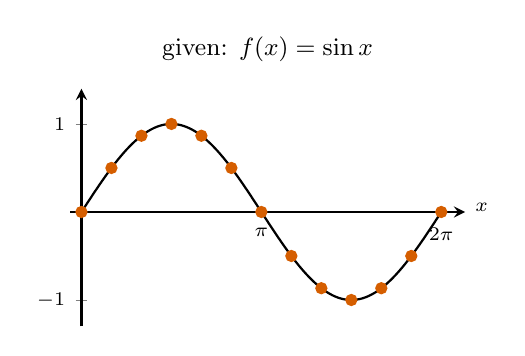
\begin{tikzpicture}
\begin{axis}[width=6.6cm,height=4.6cm,axis lines=middle,xmin=-0.2,xmax=6.7,ymin=-1.3,ymax=1.4,
  xtick={0,3.1416,6.2832},xticklabels={$0$,$\pi$,$2\pi$},ytick={-1,1},
  thick,tick label style={font=\scriptsize},title={\small given: $f(x)=\sin x$},
  xlabel={$x$},xlabel style={at={(1,0.5)},anchor=west,font=\scriptsize}]
\addplot[black,domain=0:6.2832,samples=120] {sin(deg(x))};
\addplot[only marks,mark=*,hl,mark size=1.8pt] coordinates {(0.0000,0.0000) (0.5236,0.5000) (1.0472,0.8660) (1.5708,1.0000) (2.0944,0.8660) (2.6180,0.5000) (3.1416,0.0000) (3.6652,-0.5000) (4.1888,-0.8660) (4.7124,-1.0000) (5.2360,-0.8660) (5.7596,-0.5000) (6.2832,0.0000)};
\end{axis}
\end{tikzpicture}

\scriptsize \textbf{---} formula \quad \textcolor{hl}{$\bullet$} data on a grid, $h=\pi/6$
\end{column}
\begin{column}{0.49\textwidth}
\centering
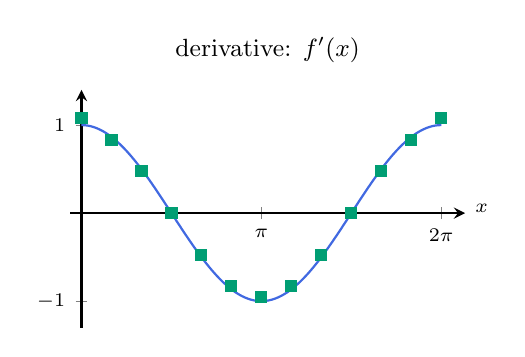
\begin{tikzpicture}
\begin{axis}[width=6.6cm,height=4.6cm,axis lines=middle,xmin=-0.2,xmax=6.7,ymin=-1.3,ymax=1.4,
  xtick={0,3.1416,6.2832},xticklabels={$0$,$\pi$,$2\pi$},ytick={-1,1},
  thick,tick label style={font=\scriptsize},title={\small derivative: $f'(x)$},
  xlabel={$x$},xlabel style={at={(1,0.5)},anchor=west,font=\scriptsize}]
\addplot[accent,domain=0:6.2832,samples=120] {cos(deg(x))};
\addplot[only marks,mark=square*,gr,mark size=1.8pt] coordinates {(0.0000,1.0829) (0.5236,0.8270) (1.0472,0.4775) (1.5708,0.0000) (2.0944,-0.4775) (2.6180,-0.8270) (3.1416,-0.9549) (3.6652,-0.8270) (4.1888,-0.4775) (4.7124,0.0000) (5.2360,0.4775) (5.7596,0.8270) (6.2832,1.0829)};
\end{axis}
\end{tikzpicture}

\scriptsize \textcolor{accent}{\textbf{---}} SymPy (exact) \quad \textcolor{gr}{$\blacksquare$} finite differences
\end{column}
\end{columns}

\vspace{0.6em}
\centering
\cbox{accent!12}{\text{Next: same two routes, but now the \textbf{unknown} is the function } y(t) \text{ itself.}}
\end{frame}

% ------------------------------------------------------------
\begin{frame}{Ordinary differential equations: order and initial conditions}
\small
An \textbf{ordinary differential equation} (ODE) links an unknown $y(t)$ to its derivatives.
\textbf{Order} = the highest derivative that appears.

\vspace{0.4em}
\begin{columns}[T]
\begin{column}{0.48\textwidth}
\begin{block}{First order: one initial condition}
\[ y'(t) = F\big(t, y\big), \quad y(t_0) = y_0 \]
\footnotesize
e.g.\ $y' + \tfrac12 y = \sin t,\ \ y(0)=1$\\[2pt]
General solution has \textbf{one} constant $C_1$.
\end{block}
\end{column}
\begin{column}{0.48\textwidth}
\begin{block}{Second order: two initial conditions}
\[ y''(t) = F\big(t, y, y'\big), \quad y(t_0) = y_0,\ y'(t_0) = y'_0 \]
\footnotesize
e.g.\ $y'' + 2y' + 5y = 0,\ \ y(0)=1,\ y'(0)=0$\\[2pt]
\textbf{Two} constants $C_1, C_2$: start position \emph{and} velocity.
\end{block}
\end{column}
\end{columns}

\vspace{0.6em}
\footnotesize
\begin{itemize}
\item The equation alone gives a \textbf{family} of solutions; the initial conditions pick \textbf{one}.
\end{itemize}

\vspace{0.3em}
\centering
\cbox{accent!12}{\text{order } n \;\Rightarrow\; n \text{ constants} \;\Rightarrow\; n \text{ initial conditions}}
\end{frame}

\end{document}
